\documentclass{ximera}
\graphicspath{  %% When looking for images,
{./}            %% look here first,
{./pictures/}   %% then look for a pictures folder,
{../pictures/}  %% which may be a directory up.
{../../pictures/}  %% which may be a directory up.
{../../../pictures/}  %% which may be a directory up.
{../../../../pictures/}  %% which may be a directory up.
}

\usepackage{listings}
%\usepackage{circuitikz}
\usepackage{xcolor}
\usepackage{amsmath,amsthm}
\usepackage{subcaption}
\usepackage{graphicx}
\usepackage{tikz}
%\usepackage{tikz-3dplot}
\usepackage{amsfonts}
%\usepackage{mdframed} % For framing content
%\usepackage{tikz-cd}

  \renewcommand{\vector}[1]{\left\langle #1\right\rangle}
  \newcommand{\arrowvec}[1]{{\overset{\rightharpoonup}{#1}}}
  \newcommand{\ro}{\texttt{R}}%% row operation
  \newcommand{\dotp}{\bullet}%% dot product
  \renewcommand{\l}{\ell}
  \let\defaultAnswerFormat\answerFormatBoxed
  \usetikzlibrary{calc,bending}
  \tikzset{>=stealth}
  




%make a maroon color
\definecolor{maroon}{RGB}{128,0,0}
%make a dark blue color
\definecolor{darkblue}{RGB}{0,0,139}
%define the color fourier0 to be the maroon color
\definecolor{fourier0}{RGB}{128,0,0}
%define the color fourier1 to be the dark blue color
\definecolor{fourier1}{RGB}{0,0,139}
%define the color fourier 1t to be the light blue color
\definecolor{fourier1t}{RGB}{173,216,230}
%define the color fourier2 to be the dark green color
\definecolor{fourier2}{RGB}{0,100,0}
%define teh color fourier2t to be the light green color
\definecolor{fourier2t}{RGB}{144,238,144}
%define the color fourier3 to be the dark purple color
\definecolor{fourier3}{RGB}{128,0,128}
%define the color fourier3t to be the light purple color
\definecolor{fourier3t}{RGB}{221,160,221}
%define the color fourier0t to be the red color
\definecolor{fourier0t}{RGB}{255,0,0}
%define the color fourier4 to be the orange color
\definecolor{fourier4}{RGB}{255,165,0}
%define the color fourier4t to be the darker orange color
\definecolor{fourier4t}{RGB}{255,215,0}
%define the color fourier5 to be the yellow color
\definecolor{fourier5}{RGB}{255,255,0}
%define the color fourier5t to be the darker yellow color
\definecolor{fourier5t}{RGB}{255,255,100}
%define the color fourier6 to be the green color
\definecolor{fourier6}{RGB}{0,128,0}
%define the color fourier6t to be the darker green color
\definecolor{fourier6t}{RGB}{0,255,0}

%New commands for this doc for errors in copying
\newcommand{\eigenvar}{\lambda}
%\newcommand{\vect}[1]{\mathbf{#1}}
\renewcommand{\th}{^{\text{th}}}
\newcommand{\st}{^{\text{st}}}
\newcommand{\nd}{^{\text{nd}}}
\newcommand{\rd}{^{\text{rd}}}
\newcommand{\paren}[1]{\left(#1\right)}
\newcommand{\abs}[1]{\left|#1\right|}
\newcommand{\R}{\mathbb{R}}
\newcommand{\C}{\mathbb{C}}
\newcommand{\Hilb}{\mathbb{H}}
\newcommand{\qq}[1]{\text{#1}}
\newcommand{\Z}{\mathbb{Z}}
\newcommand{\N}{\mathbb{N}}
\newcommand{\q}[1]{\text{``#1''}}
%\newcommand{\mat}[1]{\begin{bmatrix}#1\end{bmatrix}}
\newcommand{\rref}{\text{reduced row echelon form}}
\newcommand{\ef}{\text{echelon form}}
\newcommand{\ohm}{\Omega}
\newcommand{\volt}{\text{V}}
\newcommand{\amp}{\text{A}}
\newcommand{\Seq}{\textbf{Seq}}
\newcommand{\Poly}{\textbf{P}}
\renewcommand{\quad}{\text{    }}
\newcommand{\roweq}{\simeq}
\newcommand{\rowop}{\simeq}
\newcommand{\rowswap}{\leftrightarrow}
\newcommand{\Mat}{\textbf{M}}
\newcommand{\Func}{\textbf{Func}}
\newcommand{\Hw}{\textbf{Hamming weight}}
\newcommand{\Hd}{\textbf{Hamming distance}}
\newcommand{\rank}{\text{rank}}
\newcommand{\longvect}[1]{\overrightarrow{#1}}
% Define the circled command
\newcommand{\circled}[1]{%
  \tikz[baseline=(char.base)]{
    \node[shape=circle,draw,inner sep=2pt,red,fill=red!20,text=black] (char) {#1};}%
}

% Define custom command \strikeh that just puts red text on the 2nd argument
\newcommand{\strikeh}[2]{\textcolor{red}{#2}}

% Define custom command \strikev that just puts red text on the 2nd argument
\newcommand{\strikev}[2]{\textcolor{red}{#2}}

%more new commands for this doc for errors in copying
\newcommand{\SI}{\text{SI}}
\newcommand{\kg}{\text{kg}}
\newcommand{\m}{\text{m}}
\newcommand{\s}{\text{s}}
\newcommand{\norm}[1]{\left\|#1\right\|}
\newcommand{\col}{\text{col}}
\newcommand{\sspan}{\text{span}}
\newcommand{\proj}{\text{proj}}
\newcommand{\set}[1]{\left\{#1\right\}}
\newcommand{\degC}{^\circ\text{C}}
\newcommand{\centroid}[1]{\overline{#1}}
\newcommand{\dotprod}{\boldsymbol{\cdot}}
%\newcommand{\coord}[1]{\begin{bmatrix}#1\end{bmatrix}}
\newcommand{\iprod}[1]{\langle #1 \rangle}
\newcommand{\adjoint}{^{*}}
\newcommand{\conjugate}[1]{\overline{#1}}
\newcommand{\eigenvarA}{\lambda}
\newcommand{\eigenvarB}{\mu}
\newcommand{\orth}{\perp}
\newcommand{\bigbracket}[1]{\left[#1\right]}
\newcommand{\textiff}{\text{ if and only if }}
\newcommand{\adj}{\text{adj}}
\newcommand{\ijth}{\emph{ij}^\text{th}}
\newcommand{\minor}[2]{M_{#2}}
\newcommand{\cofactor}{\text{C}}
\newcommand{\shift}{\textbf{shift}}
\newcommand{\startmat}[1]{
  \left[\begin{array}{#1}
}
\newcommand{\stopmat}{\end{array}\right]}
%a command to give a name to explorations and hints and theorems
\newcommand{\name}[1]{\begin{centering}\textbf{#1}\end{centering}}
\newcommand{\vect}[1]{\vec{#1}}
\newcommand{\dfn}[1]{\textbf{#1}}
\newcommand{\transpose}{\mathsf{T}}
\newcommand{\mtlb}[2][black]{\texttt{\textcolor{#1}{#2}}}
\newcommand{\RR}{\mathbb{R}} % Real numbers
\newcommand{\id}{\text{id}}
\newcommand{\coord}[1]{\langle#1\rangle}
\newcommand{\RREF}{\text{RREF}}
\newcommand{\Null}{\text{Null}}
\newcommand{\Nullity}{\text{Nullity}}
\newcommand{\Rank}{\text{Rank}}
\newcommand{\Col}{\text{Col}}
\newcommand{\Ef}{\text{EF}}
\newcommand{\boxprod}[3]{\abs{(#1\times#2)\cdot#3}}

\author{Zack Reed}
%borrowed from Ana Davis
\title{Dot Product and Its Consequences}
\begin{document}
\begin{abstract}


\end{abstract}
\maketitle

\section*{Properties and Consequences of the Dot Product}

Now, we unpack various ways that the dot product is a significant calculation for applications in Linear Algebra.

First and foremost, the dot product provides us with means of relating the two vectors $\vec{u}$ and $\vec{v}$, in the sense of ascertaining how aligned the two vectors are. 

\begin{exploration}
   Use the following GeoGebra applet, answer the given questions.

   \begin{center}
      \geogebra{sm8ucyfw}{519}{330}
   \end{center}



   \begin{enumerate}
      \item If the projection vector $\vec{v}_\parallel$ is pointing in the same direction as $\vec{u}$, $\vec{u}\cdot\vec{v}$ is \wordChoice{
         \choice[correct]{positive}
         \choice{negative}
      }

      \item If the projection vector $\vec{v}_\parallel$ is pointing away from $\vec{u}$, $\vec{u}\cdot\vec{v}$ is \wordChoice{
         \choice{positive}
         \choice[correct]{negative}
      }

      \item Keeping in mind that the applet rounds to two decimal places, if $\vec{v}$ and $\vec{u}$ are perpendicular, then $\left\|\vec{v}_\parallel\right\|=\answer{0}$ and hence $\vec{u}\cdot\vec{v}$ is $\answer{0}$

      \item If $\vec{v}$ and $\vec{u}$ are perpendicular, then \begin{selectAll}
         \choice{$\vec{v}_\perp=\vec{u}$}
         \choice{$\vec{v}_\parallel=\vec{v}$}
         \choice[correct]{$\vec{v}_\perp=\vec{v}$}
         \choice{$\vec{v}_\parallel=\vec{u}$}
         \choice[correct]{$\vec{v}_\parallel=\vec{0}$}
      \end{selectAll}

      \item Select all that are true \begin{selectAll}
         \choice[correct]{If $\norm{\vec{u}}>\norm{\vec{v}}$, then $\norm{\vec{v}_\parallel}<\norm{\vec{u}}$.}

      \choice{If $\norm{\vec{u}}<\norm{\vec{v}}$, then $\norm{\vec{v}_\parallel}>\norm{\vec{u}}$.}
      \choice[correct]{If $\norm{\vec{u}}<\norm{\vec{v}_\parallel}$, then $\norm{\vec{v}}>\norm{\vec{u}}$.}
      \choice{If $\abs{\vec{u}\cdot\vec{v}}>1$, then neither of the vectors are unit vectors}
      \choice{If $\abs{\vec{u}\cdot\vec{v}}=1$, then $\vec{u}=\vec{v}$}
      \choice[correct]{If $\vec{u}$ and $\vec{v}$ are unit vectors and $\abs{\vec{u}\cdot\vec{v}}=-1$, then $\vec{u}=-\vec{v}$ }
      \end{selectAll}
   \end{enumerate}

\end{exploration}


As indicated by these exercises, $\vec{u}\cdot\vec{v}$ tells us information about the directional alignment of $\vec{u}$ and $\vec{v}$, for instance if both vectors are generally pointed in the same direction, in opposite directions, or more specifically if they are \emph{orthogonal}, that is, perpendicular.

Orthogonality of collections of vectors is a very very nice property, and will feature heavily in many of the applications we will consider moving forward. 

Also, you've gained some idea about the potential vagueness of information gained from the magnitude of the dot product. The scaling itself is more a feature of the magnitudes of the vectors, and so we gain the most information from the dot product if we know that the two vectors are unit vectors. If both are unit vectors, then we can ascertain how close or far apart the vectors are just by inspecting the dot product (e.g. is $\vec{u}\cdot\vec{v}$ close to $1$? $-1$? $0$?)

\begin{exploration}
   Let's look at our first nice consequence of utilizing the dot product for orthogonal projection: Orthogonal decomposition.

   This brings full circle our original motivation for determining the dot product, breaking up a vector $\vec{v}$ into the sum of two vectors $\vec{v}_\parallel$ and $\vec{v}_\perp$, where $\vec{v}_\parallel$ is in the span of $\vec{u}$ and $\vec{v}_\perp$ is orthogonal to $\vec{u}$.

   \begin{example}\label{ex:projection1}
      Find the orthogonal decomposition of $\vec{v}=\begin{bmatrix}
      4\\6
      \end{bmatrix}$, shown in the following figure, in reference to the vector $\vec{u}=\begin{bmatrix}
         6\\3
      \end{bmatrix}$. Then find the distance from the vector $\vec{v}$ to the subspace $\mbox{span}(\vec{u})$.
       
      \begin{center}
      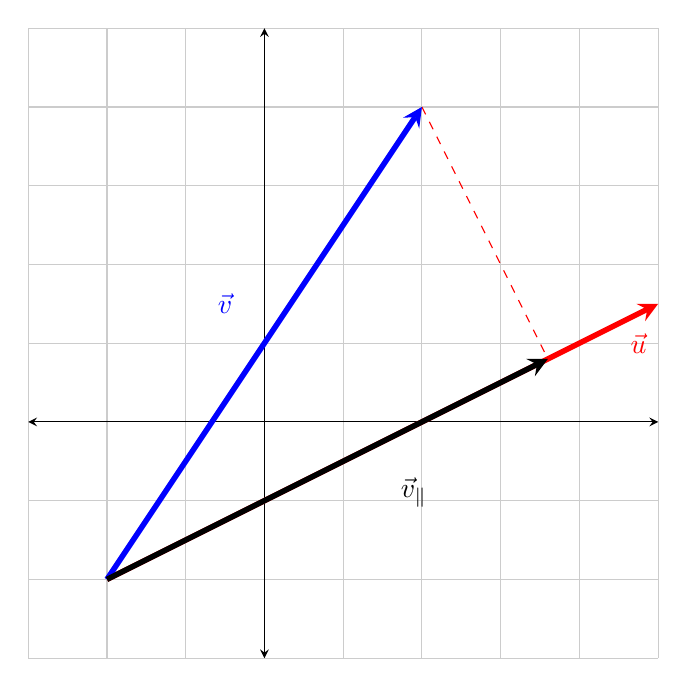
\begin{tikzpicture}
       
      \draw[thin,gray!40] (-3,-3) grid (5,5);
        \draw[<->] (-3,0)--(5,0);
        \draw[<->] (0,-3)--(0,5);
        \draw[red, dashed] (2,4)--(3.6, 0.8);
        \draw [line width=2pt, red, -stealth]  (-2,-2)--(5, 1.5);
      \draw[line width=2pt,blue,-stealth](-2, -2)--(2,4);
      \draw[line width=2pt,black,-stealth](-2, -2)--(3.6, 0.8);
      \node[blue] at (-0.5, 1.5)   (a) {$\vec{v}$};
      \node[black] at (1.9, -0.9)   (b) {$\vec{v}_{\parallel}$};
      \node[red] at (4.75,1) (c) {$\vec{u}$};
      \end{tikzpicture}
      \end{center}
       
      Orthogonally decomposing $\vec{v}$ means constructing the sum $\vec{v}=\vec{v}_\parallel+\vec{v}_\perp$, where $\vec{v}_\parallel$ is the projection of $\vec{v}$ onto $\vec{u}$ and $\vec{v}_\perp$ is orthogonal to $\vec{u}$.

      First obtaining the projection, we know that the length of the projection is $\frac{\vec{u}\cdot\vec{v}}{\norm{\vec{u}}}$. 

      $$\norm{\vec{u}}=\sqrt{\answer{36}+\answer{9}}=\answer{\sqrt{45}}.$$

      $$\vec{u}\cdot\vec{v}=\answer{24}+\answer{18}=\answer{42}.$$

      We want the projection $\vec{v}_\parallel$ to be in the direction of $\vec{u}$, so we need to find the direction vector $\vec{d}=\frac{\vec{u}}{\norm{\vec{u}}}$, and scale it by $\norm{\vec{v}_\parallel}$.

      Hence, 

      $$\vec{v}_\parallel=\frac{\answer{42}}{\answer{45}}\vec{u}\approx\begin{bmatrix}
         \answer[tolerance=.1]{5.6}\\\answer[tolerance=.1]{2.8}
      \end{bmatrix}.$$

      Then, since we have both $\vec{v}$ and $\vec{v}_\parallel$, we can find 
      
      $$\vec{v}_\perp=\vec{v}-\vec{v}_\parallel\approx \begin{bmatrix}
         \answer[tolerance=.1]{-1.6}\\\answer[tolerance=.1]{3.2}
      \end{bmatrix}.$$

      The distance from $\vec{v}$ to the subspace $\mbox{span}(\vec{u})$ is the shortest distance from $\vec{v}$ to the line in the direction of $\vec{u}$. As it turns out, that shortest distance is the length of the perpendicular vector $\vec{v}_\perp$, which is $\norm{\vec{v}_\perp}\approx\answer[tolerance=.05]{3.58}$.
      
      \end{example}

   This notion of distances to subspaces is very important for application, as we will further explore in Chapters 6 and 8. One major application that we will explore is the use of orthogonal projections to approximate vectors in application. 

   We don't need to approximate $\vec{v}$ in this case since it's just a $2D$ vector, but imagine dealing with a data set of thousands of vectors, each being thousands-dimensional vectors. There is a need in many such ``bit data'' instances to reduce the complexity of the data while retaining key features that are useable or discernible. Orthogonal projection is crucial to such endeavors.


\end{exploration}

\subsection*{Orthonormal Bases}

As hinted at in the last section, we have been treating $\vec{u}$ as if it were the first basis vector in a new coordiante system, rotated from the standard $\vec{i}$,$\vec{j}$ coordinate system.

We can even take this one step further, and construct new coordinate systems that mirror the nice properties of standard coordinate systems with basis vectors $\vec{i}$, $\vec{j}$, $\vec{k}$, .. etc. 

In particular, two key features of the standard coordinate system that make it so nice are the following:

\begin{enumerate}
   \item Each basis vector is a unit vector.
   \item All basis vectors are orthogonal to each other.
\end{enumerate}

This is the idea of an \emph{orthonormal} basis for $\RR^n$, which are very nice bases to work with. Orthonormal bases have a very nice characterization by the dot product, as we give below.

\begin{definition}
   A basis $\lbrace u_1,u_2,\ldots,u_n\rbrace$ is \emph{orthonormal} if 

   \begin{enumerate}
      \item $\vec{u}_i\cdot\vec{u}_j=0$ when $i\neq j$
      \item $\vec{u}_i\cdot\vec{u}_i=1$
   \end{enumerate}

   This second condition is the same as saying $\vec{u}_i$ is a unit vector since $\vec{v}\cdot\vec{v}=\sum_{k=1}^nv_k^2=\norm{v}^2$ for any vector $\vec{v}$.
\end{definition}

We will use orthonormal bases heavily in Chapter 6, and moving forward in the book as well.

\begin{exploration}
   Using the following GeoGebra applet, construct a new orthonormal basis for $\RR^3$ and verify that the resulting vectors satisfy the properties of an orthonormal basis.

   \begin{center}
      \geogebra{ym8uzusc}{859}{457}
   \end{center}



   \begin{hint}\name{One Possible Solution}

      While you should choose your own vectors, we will give an example starting with the vector $\vec{v}=\begin{bmatrix}
         .714\\-.645\\.273
      \end{bmatrix}$. Once $\vec{v}$ is locked in, notice that what remains orthogonal to $\vec{v}$ in $\RR^3$ is a plane. Hence, the new possible vector $\vec{w}$ rotates around the plane orthogonal to $\vec{v}$.

      Any such vector $\vec{w}$ lying on the resulting plane will suffice, such as the vector $\vec{w}=\begin{bmatrix}
         -.698\\-.688\\.199
      \end{bmatrix}$.
  
   
   Once $\vec{w}$ is locked in, all that remains in $\RR^3$ is a line, determined by only a single remaining vector $\vec{u}=\begin{bmatrix}
      .059\\-.332\\-.941
   \end{bmatrix}$ (or its negative).

   To check that these vectors comprise an orthonormal basis for $\RR^3$, we check their dot products for orthonormality. 

   This can be done efficiently by writing the basis as the columns of a $3\times 3$ matrix $B$, and iterating the dot product through all possible pairs of columns (which we can do with a for loop)

   \begin{verbatim}
   B=[.714 -.698 .059;
   -.645 -.688 -.332;
   .273 .199 -.941]

   for i=1:3
   for j=1:3
   i
   j
   dot_prod=dot(B(:,i),B(:,j))
   end
   end
   \end{verbatim}

   Because of rounding error, this will produce dot products such as $-2.5\times 10^{-5}$, $.9992$, $-6.27\times10^{-4}$, these should all be interpreted as $0$ or $1$.

\end{hint}

\end{exploration}

Finally, we give some properties of the dot product. These essentially establish the dot product as analogous to scalar multiplication. That is, it distributes across addition, scalar multiplication, is symmetric, and has other nice properties.

\begin{theorem}\label{th:dotproductproperties} The following properties hold for
   vectors $\vec{u}$, $\vec{v}$ and $\vec{w}$ in $\RR^n$ and scalar
   $k$ in $\RR$.
   \begin{enumerate}
   \item\label{item:commutative}
     $\vec{u}\dotp\vec{v}=\vec{v}\dotp\vec{u}$
      
   \item\label{item:distributive} $(\vec{u}+\vec{v})\dotp \vec{w}=\vec{u}\dotp \vec{w}+\vec{v}\dotp \vec{w}$
      
   \item\label{item:distributive-again} $\vec{u}\dotp (\vec{v}+\vec{w})=\vec{u}\dotp\vec{v}+\vec{u}\dotp \vec{w}$
      
   \item\label{item:scalar} $(k\vec{u})\dotp \vec{v}=k(\vec{u}\dotp\vec{v})=\vec{u}\dotp (k\vec{v})$
      
   \item \label{item:positive} $\vec{u}\dotp\vec{u}\geq 0$, and $\vec{u}\dotp\vec{u}=0$ if and only if $\vec{u}={\bf 0}$.
      
   \item \label{item:norm}
     $\norm{\vec{u}}^2=\vec{u}\dotp\vec{u}$
   \end{enumerate}
 \end{theorem}

\section*{Source References}

\begin{enumerate}
   \item The GeoGebra applet is derivative of an applet used on \href{http://mathinsight.org/applet/dot_product_projection}{this website} (link). 
   
   Nykamp DQ, “The dot product as projection.” From \emph{Math Insight}. http://mathinsight.org/applet/dot\_product\_projection
\end{enumerate}

\end{document}
    Suppose $\vec{d}$ is a direction vector for $l$.  Then $\vec{v}_
    {\parallel}=k\vec{d}$ for some scalar $k$.  Our goal is to find $k$. 
    \begin{align*}\vec{v}\dotp\vec{d}&=(\vec{v}_{\parallel}+\vec{v}_{\perp})\dotp\vec{d}\\
    &=(k\vec{d}+\vec{v}_{\perp})\dotp\vec{d}\\
    &=k\vec{d}\dotp\vec{d}+\vec{v}_{\perp}\dotp\vec{d}\\
    &=k\norm{\vec{d}}^2+0\\
    &=k\norm{\vec{d}}^2
    \end{align*}
    We conclude that $$k=\frac{\vec{v}\dotp\vec{d}}{\norm{\vec{d}}^2}$$
    and $$\vec{v}_{\parallel}=k\vec{d}=\left(\frac{\vec{v}\dotp\vec{d}}{\norm{\vec{d}}^2}\right)\vec{d}$$
     
    The vector $\vec{v}_{\parallel}=\left(\frac{\vec{v}\dotp\vec{d}}{\norm{\vec{d}}^2}\right)\vec{d}$ is called the \dfn{projection of $\vec{v}$ onto $\vec{d}$}.  In our discussion, $\vec{d}$ is a direction vector for line $l$.  So, we can also say that $\vec{v}_{\parallel}$ is the \dfn{projection of $\vec{v}$ onto $l$}.
     
    To find $\vec{v}_{\perp}$, observe that $\vec{v}_{\perp}=\vec{v}-\vec{v}_{\parallel}$.
     
     
    \begin{definition}\label{def:projection}
    Let $\vec{v}$ be a vector, and let $\vec{d}$ be a non-zero vector.  The \dfn{projection of $\vec{v}$ onto $\vec{d}$} is given by
    $$\mbox{proj}_{\vec{d}}\vec{v}=\left(\frac{\vec{v}\dotp\vec{d}}{\norm{\vec{d}}^2}\right)\vec{d}$$
    \end{definition}
     
    \begin{example}\label{ex:projection1}
    Find the projection of $\vec{v}$, shown below, onto the line given by $y=\frac{1}{2}x-1$.
     
    \begin{center}
    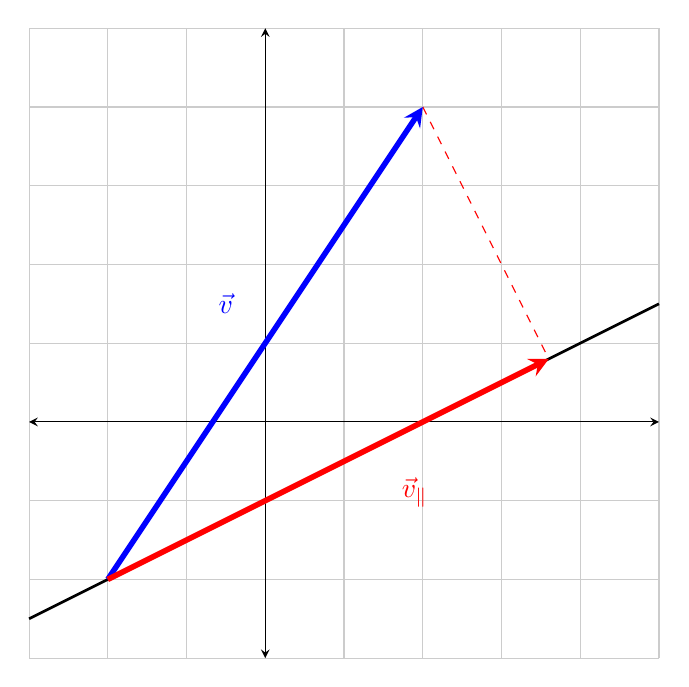
\begin{tikzpicture}
     
    \draw[thin,gray!40] (-3,-3) grid (5,5);
      \draw[<->] (-3,0)--(5,0);
      \draw[<->] (0,-3)--(0,5);
      \draw[red, dashed] (2,4)--(3.6, 0.8);
      \draw [-,line width=1pt]  (-3,-2.5)--(5, 1.5);
    \draw[line width=2pt,blue,-stealth](-2, -2)--(2,4);
    \draw[line width=2pt,red,-stealth](-2, -2)--(3.6, 0.8);
    \node[blue] at (-0.5, 1.5)   (a) {$\vec{v}$};
    \node[red] at (1.9, -0.9)   (b) {$\vec{v}_{\parallel}$};
    \end{tikzpicture}
    \end{center}
     
    \begin{explanation}
    We begin by finding vectors $\vec{v}$ and $\vec{d}$. The tail of $\vec{v}$ is located at $(-2, -2)$, and the head of $\vec{v}$ is at $(2, 4)$.  Using the ``head-tail" formula we get
    $$\vec{v}=\begin{bmatrix}2-(-2)\\4-(-2)\end{bmatrix}=\begin{bmatrix}4\\6\end{bmatrix}$$ The direction vector for the line $y=\frac{1}{2}x-1$ is $$\vec{d}=\begin{bmatrix}2\\1\end{bmatrix}$$
    We find that $\vec{v}\dotp\vec{d}=14$ and $\norm{\vec{d}}^2=5$.
    Thus $$\mbox{proj}_{\vec{d}}\vec{v}=\left(\frac{\vec{v}\dotp\vec{d}}{\norm{\vec{d}}^2}\right)\vec{d}=\frac{14}{5}\begin{bmatrix}2\\1\end{bmatrix}=\begin{bmatrix}28/5\\14/5\end{bmatrix}$$
    \end{explanation}
    \end{example}
     
    \subsection*{Distance from a Point to a Line}
     
    The shortest distance from a point to a line is the length of the perpendicular line segment dropped from the point to the line.  Vector projection formula will help us find the length of such a perpendicular.
     
    \begin{example}\label{ex:distancefrompttoline}
    Let $A(2, -1, 1)$ be a point in $\RR^3$.  Suppose line $l$ is given by parametric equations $$x=t+3$$
    $$y=-t+1$$
    $$z=t-2$$
     
    \begin{center}
    \begin{tikzpicture}
       
       \draw [-,line width=1pt]  (-3,-2.5)--(5, 1.5);
       \node[] at (5, 0.8)   (a) {$l$};
    \fill (2, 4)node[above, right]{$A(2, -1, 1)$} circle (1mm);
    \end{tikzpicture}
    \end{center}
     
    Find the distance from $A$ to $l$.
    \begin{explanation}
    We will first construct a vector $\vec{v}$ by picking an arbitrary point $B$ on $l$ to be the tail of $\vec{v}$ and using point $A$ as the head of $\vec{v}$.  An easy point to choose on line $l$ is the point $(3, 1, -2)$ that corresponds to $t=0$.  Now we have
    $$\vec{v}=\overrightarrow{BA}=\begin{bmatrix}2-3\\-1-1\\1-(-2)\end{bmatrix}=\begin{bmatrix}-1\\-2\\3\end{bmatrix}$$
     
    \begin{center}
    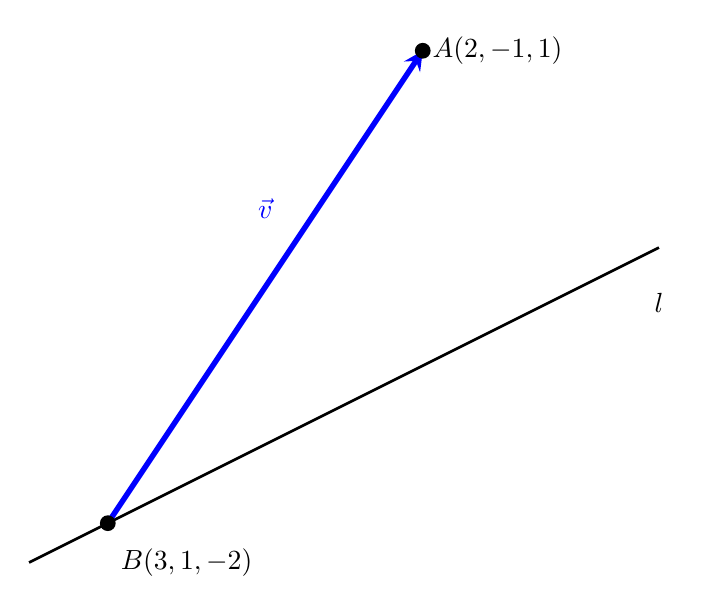
\begin{tikzpicture}
       
       \draw [-,line width=1pt]  (-3,-2.5)--(5, 1.5);
        \node[] at (5, 0.8)   (a) {$l$};
    \draw[line width=2pt,blue,-stealth](-2, -2)--(2,4);
     
    \fill (-2, -2) circle (1mm);
    \fill (2, 4)node[below, right]{$A(2, -1, 1)$} circle (1mm);
    \node[] at (-1, -2.5)   (b) {$B(3, 1, -2)$};
    \node[blue] at (0, 2)   (c) {$\vec{v}$};
    \end{tikzpicture}
    \end{center}
     
    The line has a direction vector
    $$\vec{d}=\begin{bmatrix}1\\-1\\1\end{bmatrix}$$
     
    We will now find the projection of $\overrightarrow{BA}$ onto $l$  $$\mbox{proj}_{\vec{d}} \overrightarrow{BA}=\left(\frac{\vec{v}\dotp\vec{d}}{\norm{\vec{d}}^2}\right)\vec{d}=\frac{4}{3}\begin{bmatrix}1\\-1\\1\end{bmatrix}=\begin{bmatrix}4/3\\-4/3\\4/3\end{bmatrix}$$
     
    \begin{center}
    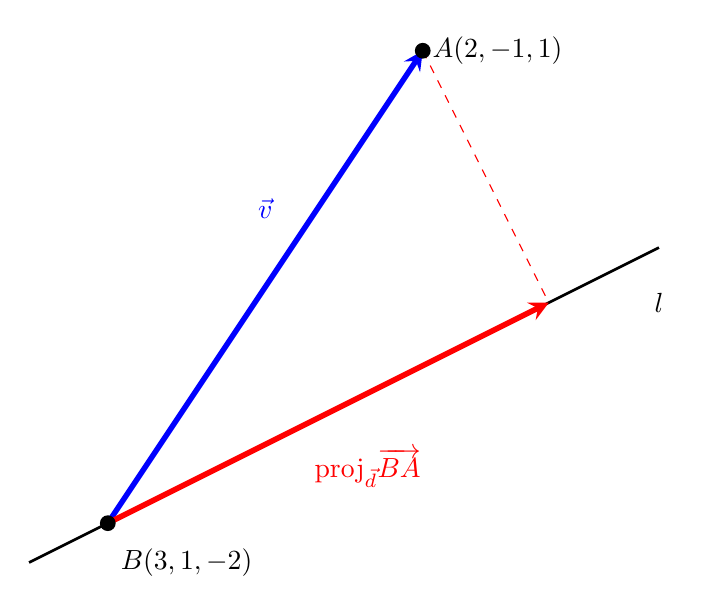
\begin{tikzpicture}
       
       \draw [-,line width=1pt]  (-3,-2.5)--(5, 1.5);
       \node[] at (5, 0.8)   (a) {$l$};
       \node[] at (-1, -2.5)   (b) {$B(3, 1, -2)$};
    \node[blue] at (0, 2)   (c) {$\vec{v}$};
    \node[red] at (1.3, -1.3)   (d) {$\mbox{proj}_{\vec{d}}\overrightarrow{BA}$};
    \draw[line width=2pt,blue,-stealth](-2, -2)--(2,4);
    \draw[line width=2pt,red,-stealth](-2, -2)--(3.6, 0.8);
    \draw[red, dashed] (2,4)--(3.6, 0.8);
    \fill (-2, -2)  circle (1mm);
    \fill (2, 4)node[above, right]{$A(2, -1, 1)$} circle (1mm);
    \end{tikzpicture}
    \end{center}
     
     
    Next, we find $\vec{v}_{\perp}$.
    $$\vec{v}_{\perp}=\vec{v}-\vec{v}_{\parallel}=\begin{bmatrix}-1\\-2\\3\end{bmatrix}-\begin{bmatrix}4/3\\-4/3\\4/3\end{bmatrix}=\begin{bmatrix}-7/3\\-2/3\\5/3\end{bmatrix}$$
     
    \begin{center}
    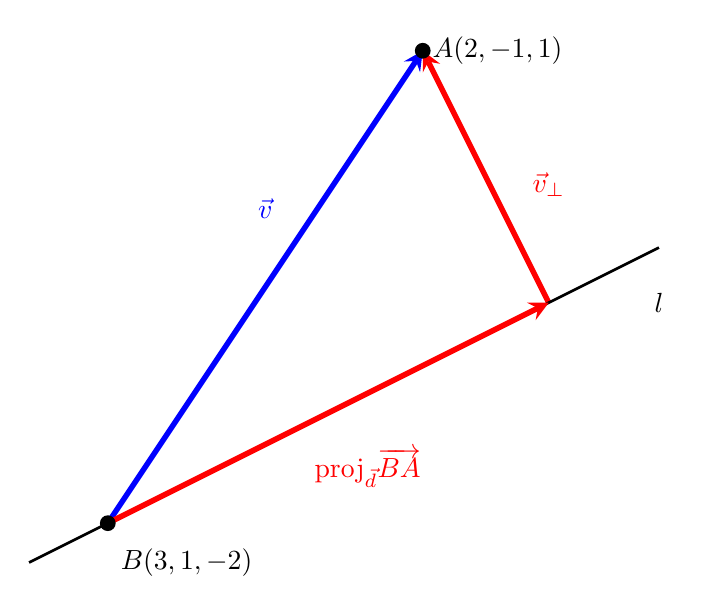
\begin{tikzpicture}
      \draw[line width=2pt,red,-stealth](3.6, 0.8)--(2,4);
       \draw [-,line width=1pt]  (-3,-2.5)--(5, 1.5);
       \node[] at (5, 0.8)   (a) {$l$};
       \node[] at (-1, -2.5)   (b) {$B(3, 1, -2)$};
    \node[blue] at (0, 2)   (c) {$\vec{v}$};
    \node[red] at (1.3, -1.3)   (d)
    {$\mbox{proj}_{\vec{d}}\overrightarrow{BA}$};
    \node[red] at (3.6, 2.3)   (e) {$\vec{v}_{\perp}$};
    \draw[line width=2pt,blue,-stealth](-2, -2)--(2,4);
    \draw[line width=2pt,red,-stealth](-2, -2)--(3.6, 0.8);
    \fill (-2, -2)  circle (1mm);
    \fill (2, 4)node[above, right]{$A(2, -1, 1)$} circle (1mm);
    \end{tikzpicture}
    \end{center}
     
     
    Finally, to find the distance between point $A$ and line $l$, we find the magnitude of $\vec{v}_{\perp}$.
    $$\norm{\vec{v}_{\perp}}=\frac{1}{3}\sqrt{49+4+25}=\frac{\sqrt{78}}{3}$$
    \end{explanation}
    \end{example}
     
     
      

\end{document}